\documentclass[11pt, a4paper]{article}
\usepackage[utf8]{inputenc}
\usepackage[margin=1.2 in]{geometry}
\usepackage{graphicx}
\usepackage[T1]{fontenc}
\usepackage{charter}
\usepackage{amsmath}
\usepackage{setspace}
\usepackage{subcaption}
\usepackage{listings}
\usepackage{color}

\graphicspath{{Assets/}}

\title{\vspace*{\fill}CSCU9V5 \\ Distributed Systems Assignment Report}
\author{Student no: 2519302}
\date{November 25\textsuperscript{th} 2018\vspace*{\fill}}
\pagenumbering{roman}
\begin{document}
\clearpage\maketitle
\thispagestyle{empty}
\newpage
\doublespacing
\setstretch{1.15}
\tableofcontents
\thispagestyle{empty}
\newpage
\singlespacing

\section{Problem Description}

This report will detail the implementation of a token passing ring node network in Java. This implementation uses RMI as the means of communicating with each node in the network and communication between each node is directed by a token passed through this network. 

The general description of the task is as such, we have a ringManager class that acts as a client which initializes a connection with the first node in the network and passes a token to that node. From there the ringMemberImpl class that acts as a server node in the network with the task of receiving the token it is passed, recording that transaction onto a file and releasing the token on to the next node in the network. Each node in the network is to record their transactions onto the same file each time, this is allowed since RMI makes blocking calls to each node.  This is done until some stopping condition is provided. Below is a diagram that outlines the network architecture for this task:

\begin{figure}[!h]
\centering
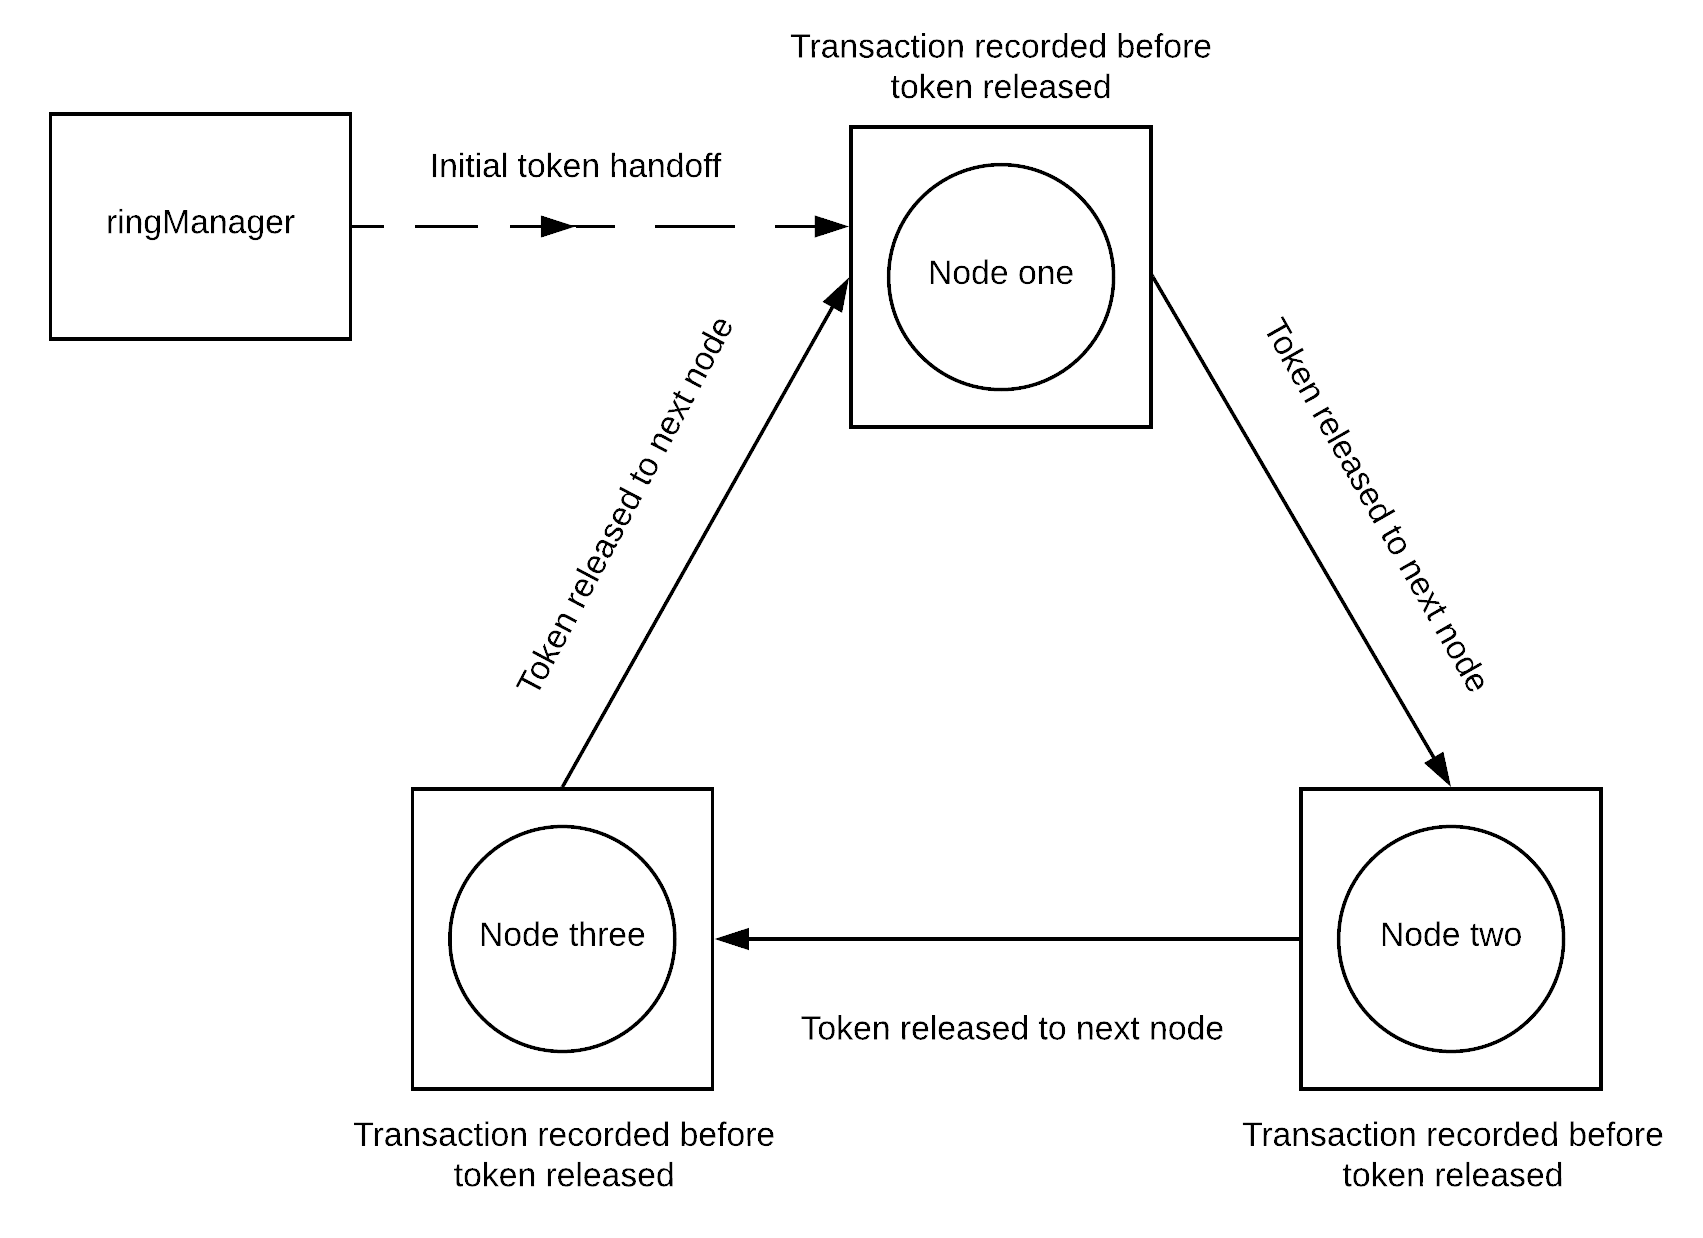
\includegraphics[scale=0.2]{ring_net}
\caption{Architecture of this ring network}
\end{figure} 

\newpage

\section{Assumptions}

In the process of implementing the solution to this project, a few assumptions were made. The assumptions made were as follows:

\begin{itemize}
\item[1] Assume that there can be multiple nodes with the same ID
\item[2] Assume that the user enters their inputs correctly
\end{itemize}
Assumption number one, is made since, if this program is run across different machines, it is possible for there to be more than one node with the same ID. This is due to the fact that each node is on a different host which as far as the program is concerned does not pose an issue upon instantiation. This raises the requirement to check both the node ID and the host of that node.

Assumption number two assumes that the user is aware of what should be entered in the command line interface. Due to this assumption, no checks are done upon user input in the command line interface. The only checks that are present for command line input are related to the number of parameters entered. 

\newpage

\section{Solution implementation}

This section of the report aims to explain the solution implemented in this project. Additionally, accompanying screenshots of how each class when instantiated in the command line will be shown to demonstrate what the program should look like before the token passing is initiated.

\begin{figure}[!h]
\centering
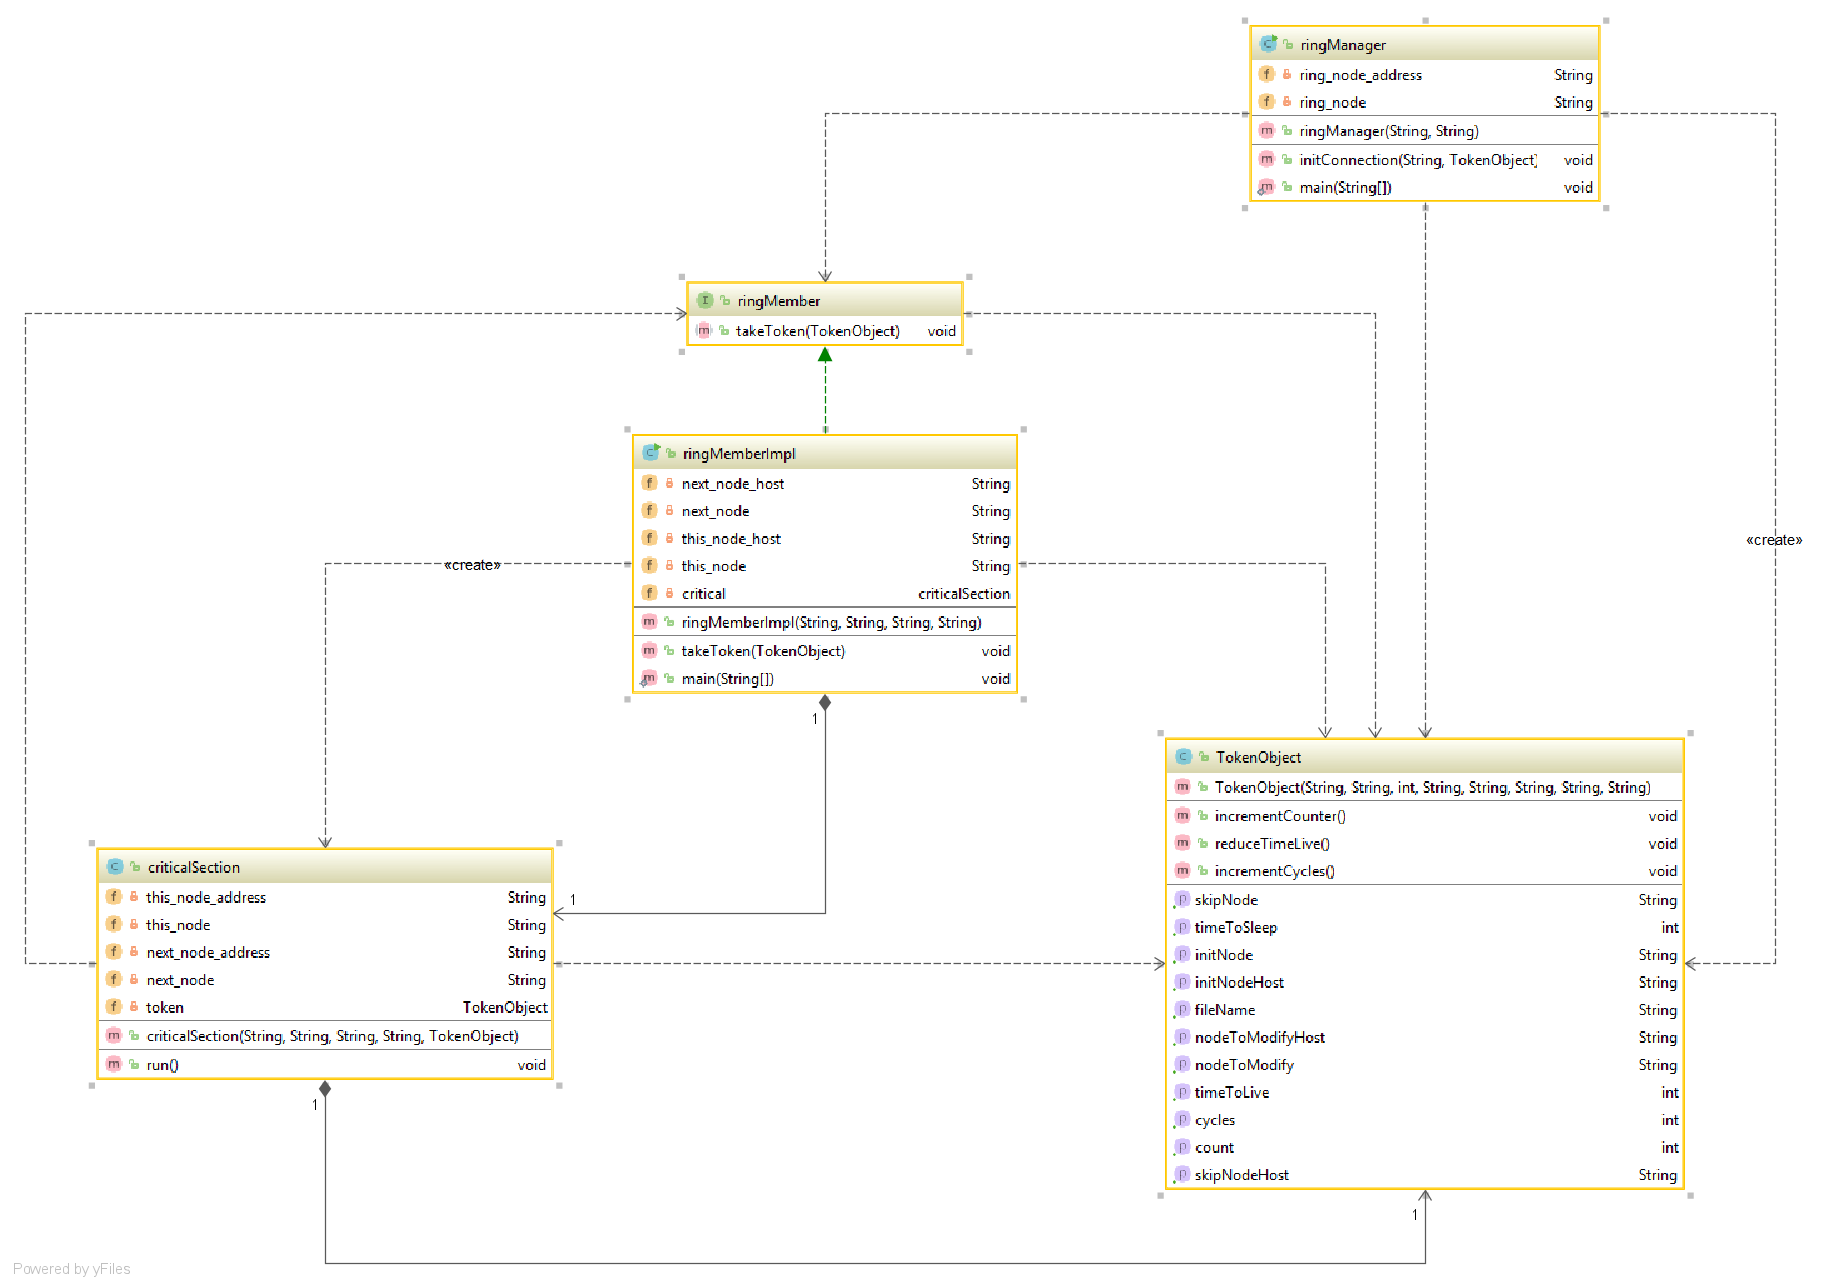
\includegraphics[scale=0.26]{class_diagram}
\caption{Class diagram}
\end{figure}

\subsection{ringManager}

The ringManager class, as mentioned before serves as the client to initialize connection to the network and passes the token to a node. In this class, we have two instance variables holding the inital node's ID and the host in which that node exists. This is so that the client can resolve the node to which it should send the token off to. The method \textit{initConnection()} serves as the function that handles initializing the connection between ringManager and the first node it sends the token to. Inside this method, we handle the clearing of the shared file for writing whenever we restart the network as well as getting a remote reference to the node and injecting the token into the network.

In the main method for the ringManager, we accept 8 parameters in the command line interface. These variables are:
\begin{itemize}
\item the host on which the initial node exists
\item the initial node ID
\item the filename(with extension) of the shared file
\item the time to live of the token (max number of passes token can take)
\item the node ID to send extra sleep to
\item the host where the extra sleep node exists
\item the node ID to skip
\item the host where the node to skip exists
\end{itemize} 
All of these variables save the first two are entered here for the sole purpose of initializing them within the token Object. This eliminates the need for each node in the network to store these variables.\\\\
Below is an example of how ringManager should look like when run in the command line, along with the arguments in their respective order:
\begin{figure}[!h]
\centering
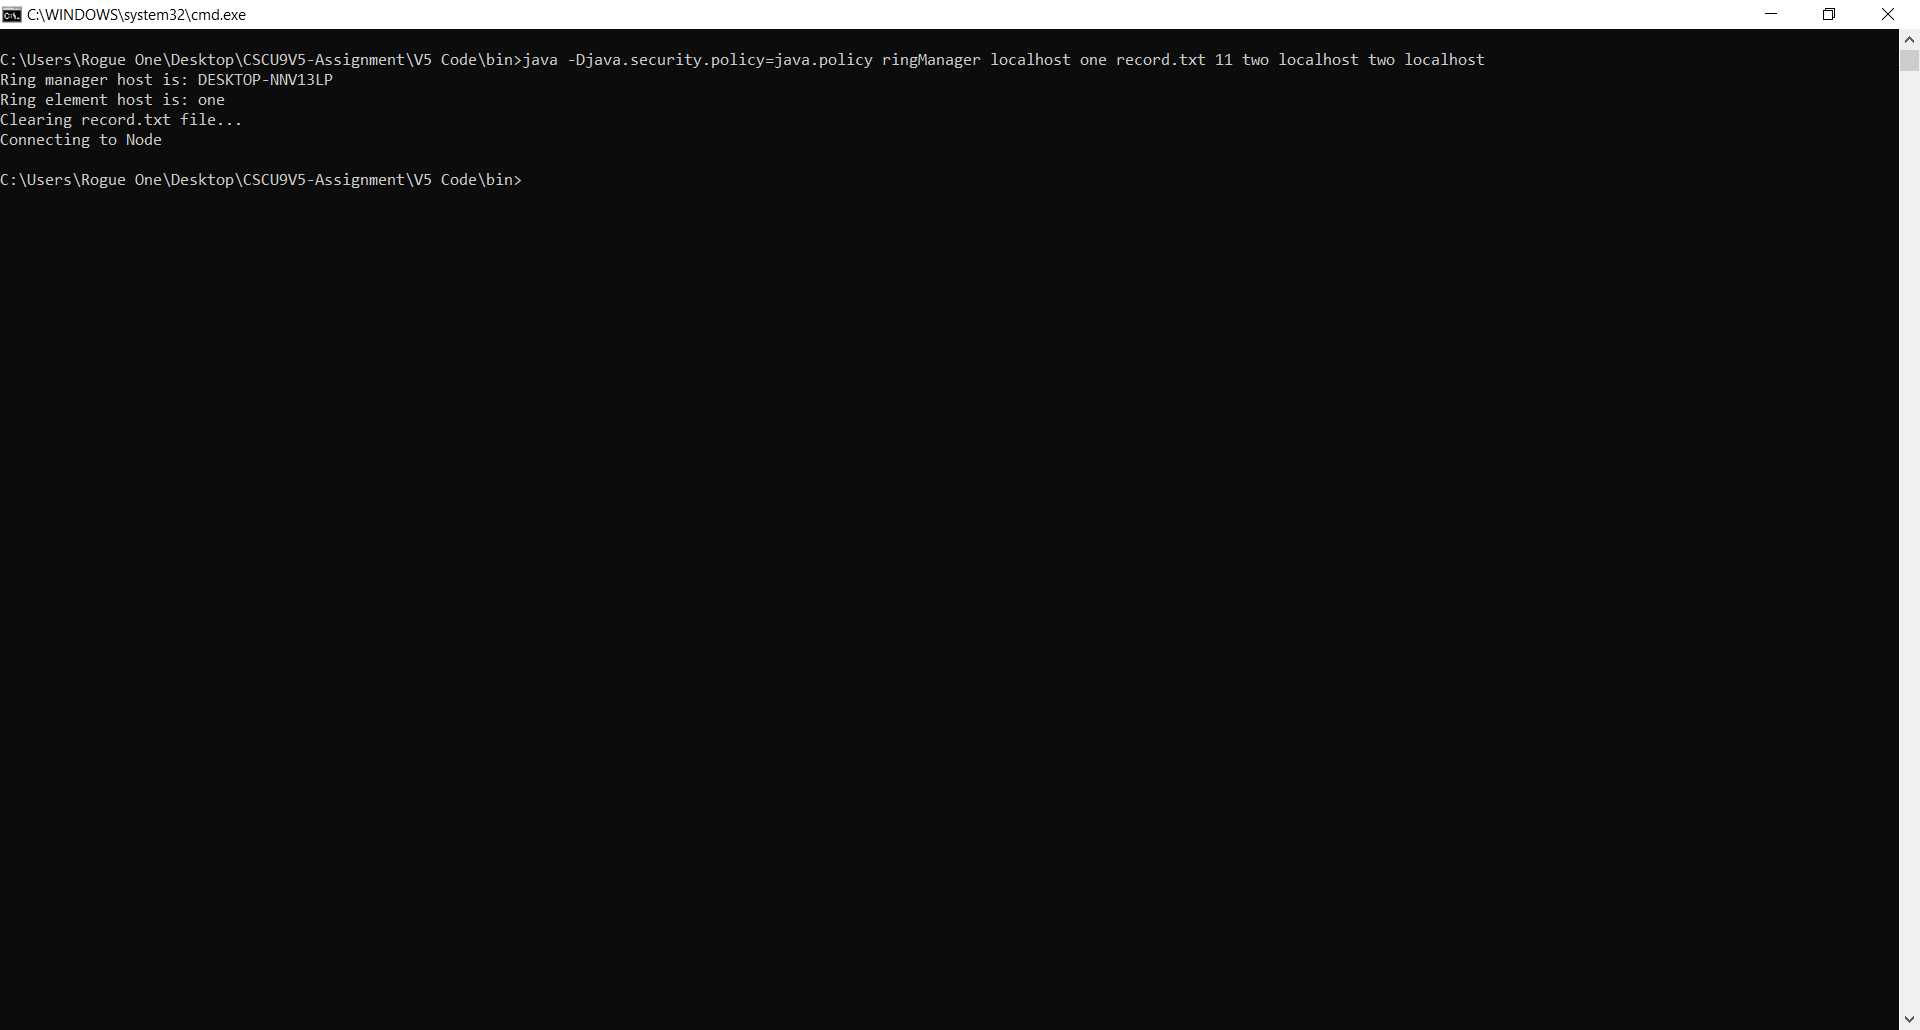
\includegraphics[scale=0.35]{ring_manager}
\caption{Example run of ringManager in Command Prompt}
\end{figure}

\subsection{ringMemberImpl}

The ringMemberImpl class, as mentioned in the first section, serves as each server node. This class implements the ringMember interface. This implementation is to allow for RMI method calls to the node. In this class resides the takeToken() method which deals with the receiving of the token and passing the token on to the next node in the network. This is representative of the critical section in this program, however due to the nature of RMI calls being blocking calls, the actual critical section is implemented as a separate Thread which is started within this method body. The main method of this class is fairly simple, with the 4 variables passed in as command line arguments:
\begin{itemize}
\item the node ID of the current node to initialize
\item the host on which to initialize this node
\item the node ID of the immediate next node
\item the host on which the immediate next node exists
\end{itemize}
Below is an example of how an instance of ringManagerImpl would look like when run using the command line:
\begin{figure}
\centering
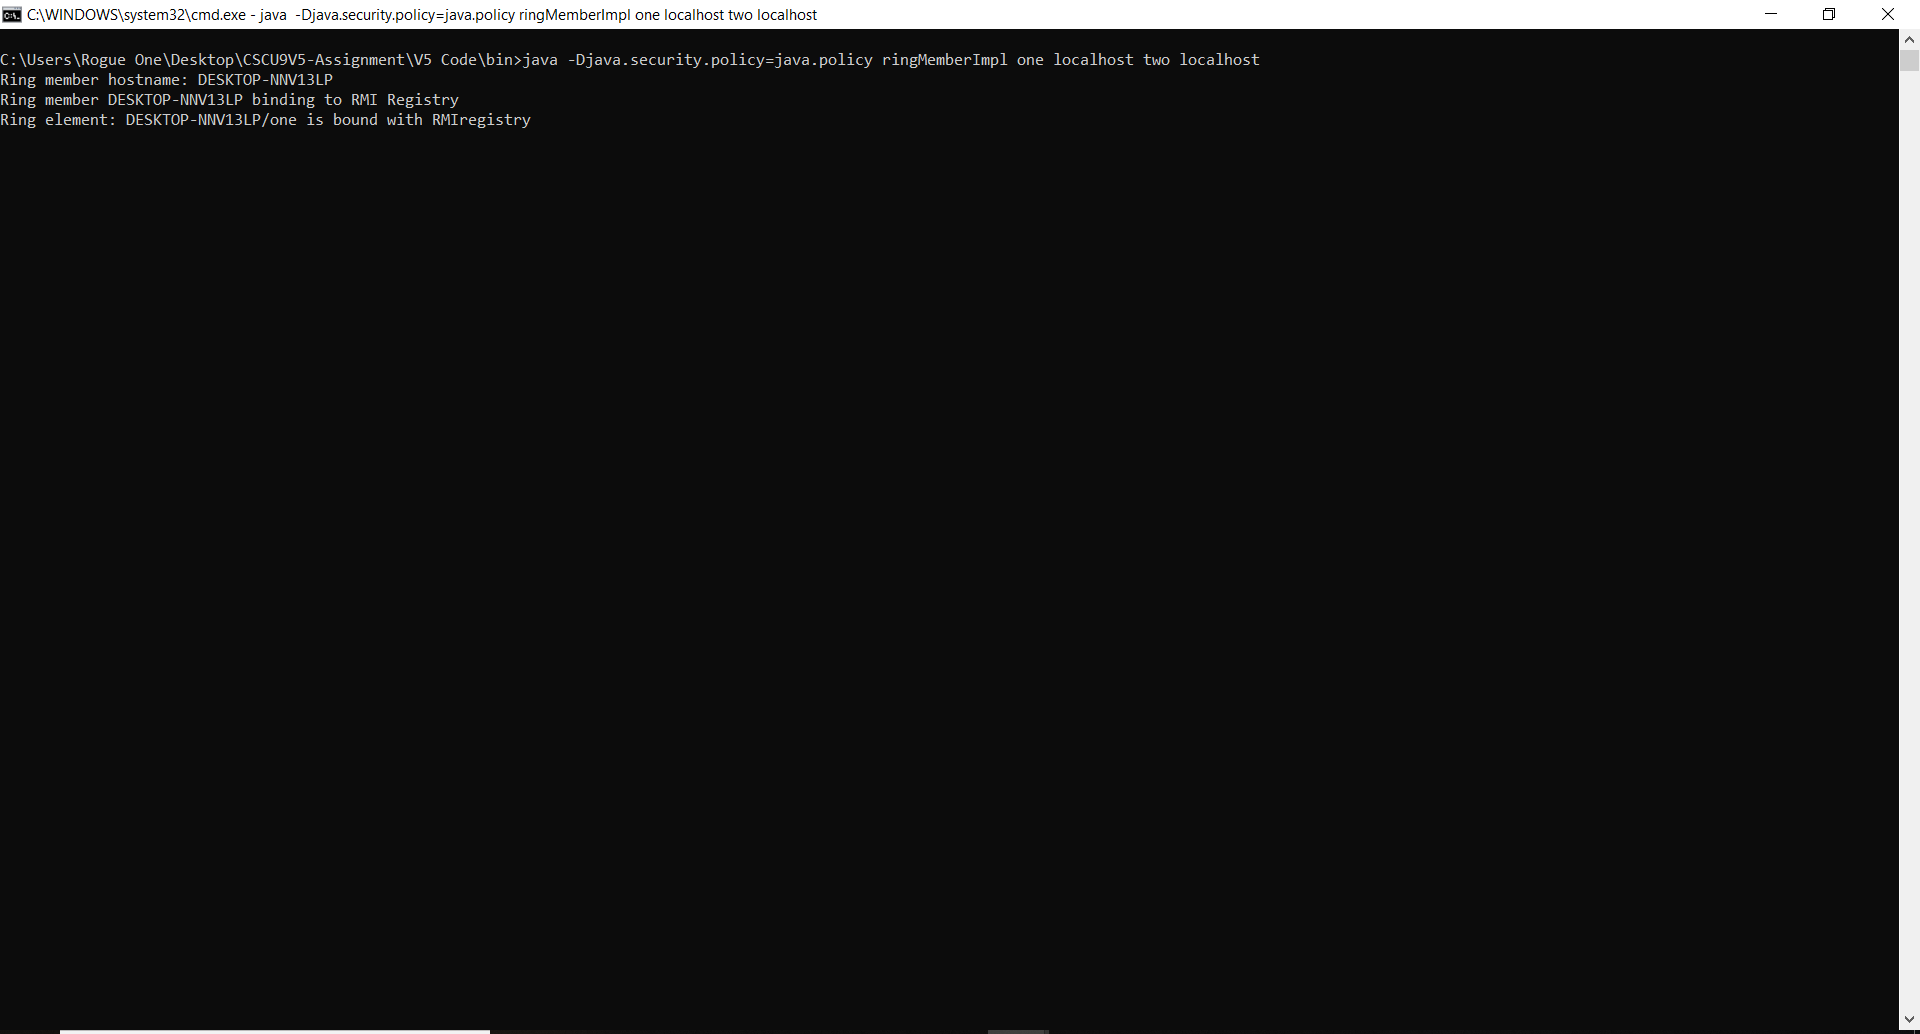
\includegraphics[scale=0.35]{ring_memberimpl_example}
\caption{Example of ringMemberImpl on Command Prompt}
\end{figure}

\subsection{ringMember}

This is an interface. This interface implements the method takeToken() which is called in the class ringMemberImpl. This interface is implemented in order to allow for RMI method calls on the node. 

\subsection{criticalSection}

The criticalSection class is the class where the actual critical section of execution is held. This class extends Thread so that it can be executed on a separate Thread in order to circumvent a deadlock situation given that RMI method calls are blocking calls. Given that this section is executed as a Thread, the run() method is implemented here. Upon running of the Thread, most of the logic regarding the activity of the node is handled here. These include, keeping track of the number of passes the token has taken through the node, keeping track of the number of cycles through the network the token has taken, logging the transaction of the token to a shared file and handling which node should be skipped and which node is getting extra time to sleep. 

\subsection{TokenObject}

The TokenObject class serves as the class that instantiates the token Object. This class contains the instance variables as passed in from the command line for ringManager. Having these variables in the token itself allows for greater ease in keeping track of where the token is and as a result, allows for easier manipulation of node activity.

\subsection{Full run of program}
\begin{figure}[!h]
\centering
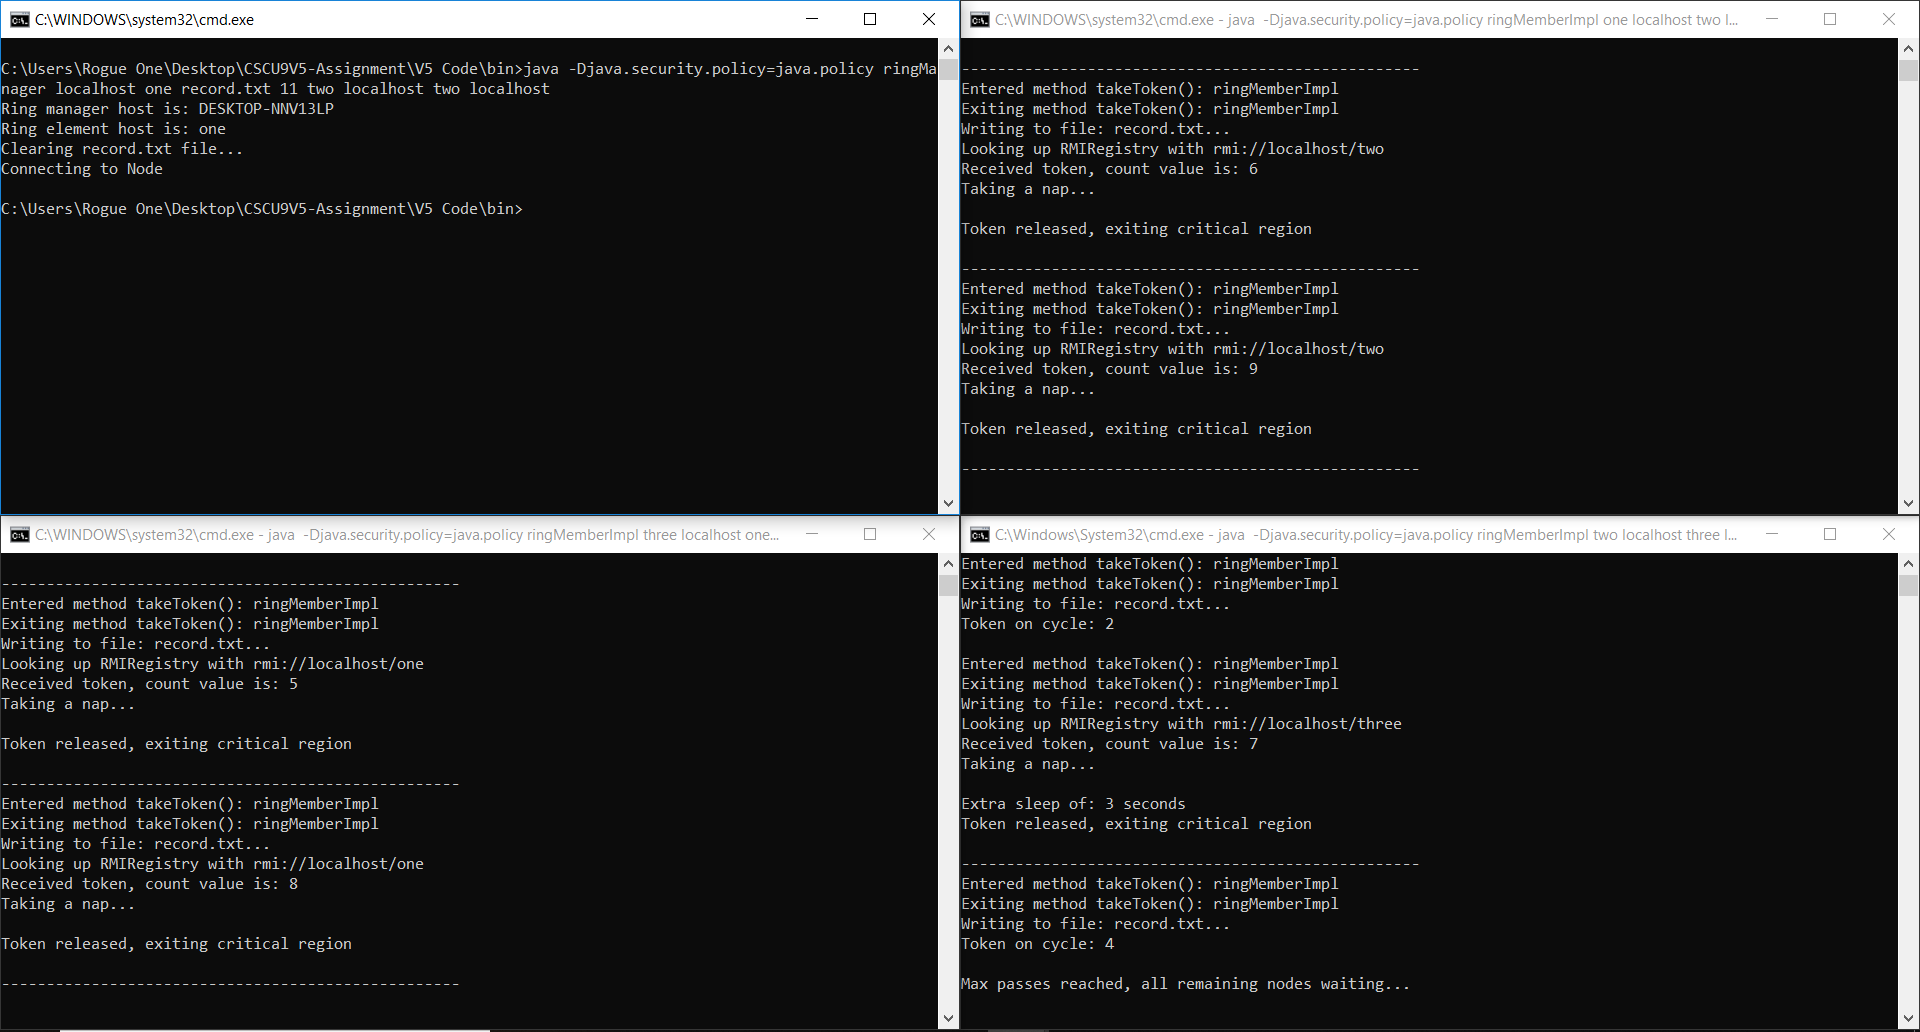
\includegraphics[scale=0.4]{full_run}
\caption{Example of a full run of the program on Command Prompt}
\end{figure}

\newpage

\section{Advanced Implementation}
This section will detail the advanced implementations as implemented in this project.

\subsection{Injecting an actual token Object which keeps a counter of how many objects it has been passed to}

Implementing an actual token Object was done by making the TokenObject class as mentioned above in Subsection 3.5. This implementation also required a change to be made to the takeToken() method in both the ringMember interface and the ringMemberImpl class where it takes in a parameter of type TokenObject. This TokenObject then stores a counter variable and a method to increment this counter. From there in the critical section, whenever the token enters a node and the critical section Thread executes, the token has its counter increased by one. This implementation in critical to the further implementations. 

\subsection{Allow user to input file name for shared file}

Implementing the file name from user input was done by accepting it in the command line run for ringManager and storing it in the TokenObject. From then it is merely passing that String variable from the token to the FileWriter in the critical section. 

\subsection{Specify number of passes a token can take in the network}

This feature was implemented by accepting a value for the number of passes a token can take in the network from the command line run for ringMember and storing it in the TokenObject. From there it is merely keeping track of the number of passes the token has taken, I personally do it by counting down the number of passes taken and when the max number of passes has reduced to zero, the token is not passed anymore and the remaining nodes are left to wait.

\subsection{Direct the n\textsuperscript{th} node to get extra sleep}

The n\textsuperscript{th} node is directed to get extra sleep by accepting the values for the node id and the host where that node exists into the TokenObject. From there a check is made in the critical section if the node the token is in is the node that is to get extra sleep. If that check resolves to true, the node is allocated a sleep time already initialized in the TokenObject and the node will print out a String stating the amount of sleep it is getting extra. 

\subsection{Directing the m\textsuperscript{th} node to be skipped every second visit of the token}

The m\textsuperscript{th} node is skipped by having the token keep track of which cycle it is on and which token it is to skip. The token keeps track of the cycle it is on by keeping track of the first node it passes and increments a counter when it passes that node again. Then in the critical section, a check can be made if the token is on an even number cycle \textbf{and} the node is the node to be skipped. If that condition resolves as true, the node does not increment the counter in the token and just passes the token on to the next node in the network.

\appendix

\newpage
\definecolor{my_magenta}{rgb}{0.8, 0.2, 0.4}
\definecolor{my_blue}{rgb}{0.33, 0.56, 0.93}
\definecolor{my_gray}{rgb}{0.5,0.5,0.5}
\lstset{ %
  backgroundcolor=\color{white},   % choose the background color
  basicstyle=\small\ttfamily,        % size of fonts used for the code
  breaklines=true,                 % automatic line breaking only at whitespace
  captionpos=b,                    % sets the caption-position to bottom
  commentstyle=\color{my_gray},    % comment style
  escapeinside={\%*}{*)},          % if you want to add LaTeX within your code
  keywordstyle=\color{my_magenta},       % keyword style
  stringstyle=\color{my_blue},     % string literal style
  showspaces=false,
  showtabs=false,
  showstringspaces=false,
  tabsize=3,					   % set tabsize in listing 
}

\section{Code Listings}
\subsection{ringManager.java}
\lstinputlisting[language=Java]{ringManager.java}
\newpage
\subsection{ringMemberImpl.java}
\lstinputlisting[language=Java]{ringMemberImpl.java}
\newpage
\subsection{ringMember.java}
\lstinputlisting[language=Java]{ringMember.java}
\newpage
\subsection{criticalSection.java}
\lstinputlisting[language=Java]{criticalSection.java}
\newpage
\subsection{TokenObject.java}
\lstinputlisting[language=Java]{TokenObject.java}
\end{document}
